% ==========================================================================
% RCSS CAMPUS NETWORK -- PROJECT REPORT
% Design and Implementation of the RCSS Campus Network Using Cisco Packet Tracer
% Compile with pdflatex (twice or three times, for the ToC and cross-references).
% ==========================================================================
\documentclass[11pt,a4paper]{article}

% --- Fonts: Times New Roman (TeX Gyre Termes metrics) for text and math ---
\usepackage[T1]{fontenc}
\usepackage{newtxtext}
\usepackage{newtxmath}
\renewcommand{\ttdefault}{cmtt}

% --- Page layout ---
\usepackage[a4paper,margin=22mm,headheight=15pt]{geometry}
\usepackage{microtype}
\usepackage{fancyhdr}
\usepackage{titlesec}

% --- Tables, figures, code ---
\usepackage{booktabs}
\usepackage{longtable}
\usepackage{array}
\usepackage{graphicx}
\usepackage{float}
\usepackage{caption}
\usepackage{pdflscape}
\usepackage{listings}
\usepackage{amsmath}
\usepackage{enumitem}
\usepackage{xcolor}

% --- Hyperlinks: blue, clickable Table of Contents ---
\definecolor{linkblue}{RGB}{0,0,190}
\usepackage[colorlinks=true,linkcolor=linkblue,urlcolor=linkblue,citecolor=linkblue]{hyperref}
\hypersetup{
  pdftitle={Design and Implementation of the RCSS Campus Network Using Cisco Packet Tracer},
  pdfsubject={Hardware and Networking Project Report},
  pdfauthor={Abhishek Vincent},
  bookmarksnumbered=true
}

% --- Section formatting ---
\titleformat{\section}{\normalfont\Large\bfseries}{\thesection}{0.75em}{}
\titleformat{\subsection}{\normalfont\large\bfseries}{\thesubsection}{0.6em}{}
\titleformat{\subsubsection}{\normalfont\normalsize\bfseries}{\thesubsubsection}{0.6em}{}
\titlespacing*{\section}{0pt}{14pt}{6pt}
\titlespacing*{\subsection}{0pt}{10pt}{4pt}
\setcounter{secnumdepth}{3}
\setcounter{tocdepth}{2}
\renewcommand{\arraystretch}{1.15}
\setlength{\tabcolsep}{3pt}

% --- Header / footer ---
\pagestyle{fancy}
\fancyhf{}
\lhead{\small RCSS Campus Network}
\rhead{\small \leftmark}
\cfoot{\thepage}
\renewcommand{\headrulewidth}{0.4pt}
\renewcommand{\footrulewidth}{0pt}

% --- Caption style ---
\captionsetup{font=small,labelfont=bf,labelsep=period,width=0.95\textwidth}

% --- Code listing style (Cisco CLI) ---
\definecolor{codebg}{RGB}{246,248,251}
\definecolor{codeframe}{RGB}{200,209,220}
\lstdefinestyle{cli}{
  basicstyle=\ttfamily\small,
  backgroundcolor=\color{codebg},
  frame=single,
  rulecolor=\color{codeframe},
  breaklines=true,
  columns=fullflexible,
  keepspaces=true,
  showstringspaces=false,
  xleftmargin=4pt,
  xrightmargin=4pt,
  aboveskip=8pt,
  belowskip=8pt
}
\lstset{style=cli}

% --- Table helper for wide tables ---
\newcolumntype{L}[1]{>{\raggedright\arraybackslash}p{#1}}
\newcolumntype{C}[1]{>{\centering\arraybackslash}p{#1}}

\newcommand{\placeholder}[1]{\textbf{[#1]}}
\newcommand{\figref}[1]{Figure~\ref{#1}}
\newcommand{\shot}[1]{\texttt{\footnotesize screenshots/}\newline\texttt{\footnotesize #1}}

\begin{document}

% ==========================================================================
% COVER PAGE
% ==========================================================================
\begin{titlepage}
\centering
\vspace*{4mm}

% --- College emblem ---

\includegraphics[width=3.6cm]{rajagiri_emblem.png}

\vspace{6mm}
{\Large\bfseries Rajagiri College of Social Sciences (Autonomous)\par}
\vspace{1.5mm}
{\large Kalamassery, Kochi, Kerala\par}

\vspace{11mm}
% --- Project title ---
{\Large\bfseries Design and Implementation of the\\[2mm]
RCSS Campus Network Using Cisco Packet Tracer\par}

\vspace{5mm}
{\large A Project Report on VLAN Segmentation, 802.1Q Trunking,\\[1mm]
Router-on-a-Stick Routing and DHCP Addressing\par}

\vspace{9mm}
{\large Project Report submitted to Mr.~Diljith K Benny\par}

\vspace{11mm}
{\large\bfseries Submitted by\par}
\vspace{3mm}
{\large Abhishek Vincent\par}

\vfill
{\small
\begin{minipage}{0.9\textwidth}
\centering
\renewcommand{\arraystretch}{1.35}
\begin{tabular}{@{}L{0.30\textwidth} L{0.58\textwidth}@{}}
\textbf{Course}          & Master of Computer Applications (MCA) \\
\textbf{Department}      & Computer Science \\
\textbf{Academic Year}   & 2026--2028 \\
\textbf{Submission Date} & 20 October 2026 \\
\end{tabular}
\end{minipage}
\par}
\end{titlepage}

\thispagestyle{empty}
\clearpage

% ==========================================================================
% ABSTRACT
% ==========================================================================
\begin{abstract}
\noindent
This report documents the design and implementation of a simulated three-building campus
network for the RCSS campus in Cisco Packet Tracer. The network is built around a single
Cisco 2911 router (\texttt{RCSS-R1}) and four Cisco 2960 switches: a core switch
(\texttt{RCSS-SW-CORE}) and one access switch per building (\texttt{RCSS-SW-ASSUMPTION},
\texttt{RCSS-SW-CARMEL}, \texttt{RCSS-SW-OLDBLOCK}). Traffic is separated into four
IEEE 802.1Q VLANs (10 Assumption, 20 Carmel, 30 Old Block lab and 40 Servers), the four
core uplinks are configured as 802.1Q trunks, and inter-VLAN routing is provided by
router-on-a-stick subinterfaces \texttt{GigabitEthernet0/0.10} to
\texttt{GigabitEthernet0/0.40} on the router's single physical uplink. Four DHCP pools
with a reserved low range (.\textit{x}.1 to .\textit{x}.20) provide automatic IPv4
addressing to clients, while the server \texttt{RCSS-SRV01} is given the static address
192.168.40.2/24 with gateway 192.168.40.1. Verification was carried out with
\texttt{show ip interface brief}, \texttt{show vlan brief}, \texttt{show interfaces trunk},
\texttt{show ip dhcp pool}, \texttt{show ip dhcp binding}, \texttt{show ip route},
\texttt{show running-config} and ICMP ping; the captured outputs confirm that all four
router subinterfaces, all four core trunks and all three building uplinks are up, that
DHCP leases were issued in the three client VLANs starting above the reserved range
while the server VLAN holds none, and that a ping to a client in the VLAN 20 subnet
returned replies. The limitations of the simulation and the evidence that
was not captured are stated explicitly in Sections 10 and 12.
\end{abstract}

\thispagestyle{empty}
\clearpage

% ==========================================================================
% TABLE OF CONTENTS
% ==========================================================================
\tableofcontents
\clearpage

\listoffigures
\clearpage

% ==========================================================================
% 1. INTRODUCTION
% ==========================================================================
\section{Introduction}

\noindent
The RCSS campus network assignment required a working, segmented campus network built
entirely in Cisco Packet Tracer. A campus of this kind does not exist as one flat
Layer 2 network in practice: each building hosts different user groups (administrative
staff, faculty, laboratory machines and shared devices), and each of those groups needs
its own logical segment, its own addressing, and its own gateway.

The report therefore moves from the physical topology (Section~\ref{sec:topology}),
through the logical VLAN and IP design (Sections~\ref{sec:logical}--\ref{sec:ipdhcp}),
to the exact configuration sequence used to build the network (Section~\ref{sec:config}),
and finally to the verification evidence collected from the live simulation
(Section~\ref{sec:verify}).

Two rules were applied while writing this report. First, every statement about the
network's behaviour is either taken from a captured command output in
\texttt{screenshots/} or is explicitly marked as a design intention that was not
independently verified. Second, the original Packet Tracer project file
\texttt{rcss-campus.pkt} was never modified during the preparation of this document;
the images in \texttt{screenshots/} are copies of the original captures.

% ==========================================================================
% 2. OBJECTIVES
% ==========================================================================
\section{Objectives}

The project was executed with the following objectives:

\begin{enumerate}[label=\textbf{\arabic*.},leftmargin=2em]
  \item Design a multi-building campus network topology joining a router, a core
        switch and three building switches.
  \item Segment the network endpoints into VLANs according to user group and function.
  \item Configure switch access ports and the 802.1Q trunk links between the core switch
        and the building switches and the router.
  \item Configure inter-VLAN routing with the router-on-a-stick method, using one
        physical interface and four tagged subinterfaces.
  \item Provide dynamic IPv4 addressing to client devices through four DHCP pools.
  \item Assign a static IPv4 address and default gateway to the campus server.
  \item Test gateway reachability and inter-VLAN / cross-building connectivity with
        ICMP.
  \item Save and document the complete configuration of every device.
\end{enumerate}

% ==========================================================================
% 3. TOOLS AND TECHNOLOGIES
% ==========================================================================
\section{Tools and Technologies}

\begin{table}[H]
\centering
\small
\caption{Technologies used in the project}
\begin{tabular}{@{}L{0.28\textwidth} L{0.66\textwidth}@{}}
\toprule
\textbf{Technology / tool} & \textbf{Role in the project} \\
\midrule
Cisco Packet Tracer       & Simulation platform used to build, configure and test the
                            network end to end. \\
Cisco 2911 router         & \texttt{RCSS-R1}; provides the default gateway for all four
                            VLANs through 802.1Q subinterfaces. \\
Cisco 2960-24TT switch    & \texttt{RCSS-SW-CORE}; terminates all four trunks and carries
                            the VLANs between buildings. \\
Cisco 2960 switches       & \texttt{RCSS-SW-ASSUMPTION}, \texttt{RCSS-SW-CARMEL},
                            \texttt{RCSS-SW-OLDBLOCK}; provide access ports for the
                            building endpoints. \\
Copper straight-through   & Physical connectivity between the router, the switches and \\
cabling                    & the end devices. \\
IPv4 subnetting (/24)     & Address plan; each VLAN receives one 192.168.\textit{x}.0/24
                            subnet. \\
VLANs (802.1Q)            & Logical Layer 2 segmentation of the four user groups. \\
IEEE 802.1Q tagging       & Carries multiple VLANs over the single physical router-to-core
                            link and over the three building uplinks. \\
Router-on-a-stick         & Inter-VLAN routing using subinterfaces on one physical
                            GigabitEthernet port. \\
DHCP                      & Automatic address assignment to the ten DHCP clients; four
                            pools with reserved low ranges. \\
ICMP (\texttt{ping})       & Connectivity verification between gateways and between
                            endpoints in different VLANs. \\
\bottomrule
\end{tabular}
\end{table}

% ==========================================================================
% 4. REQUIREMENTS AND ASSUMPTIONS
% ==========================================================================
\section{Requirements and Assumptions}

\subsection{Requirements}

The following functional requirements were derived from the campus scenario:

\begin{itemize}
  \item \textbf{Connectivity across three buildings.} The Assumption block, the Carmel
        faculty block and the Old Block laboratory must all be reachable from a single
        routed campus.
  \item \textbf{Logical segmentation.} Administrative, faculty, laboratory and server
        traffic must be separated so that a broadcast domain stays inside one user
        group, without needing separate physical equipment per group.
  \item \textbf{A default gateway in every VLAN.} Each VLAN must have exactly one
        router interface acting as the gateway for its subnet.
  \item \textbf{Automatic client addressing.} Client PCs and the printer must obtain
        their address, mask and gateway from the router rather than being configured
        manually, and the reserved low range must not be handed out.
  \item \textbf{A reachable server.} The server must carry a fixed, predictable address
        that does not change when leases are renewed and that cannot be given away by
        DHCP.
\end{itemize}

\subsection{Assumptions and scope}

\begin{itemize}
  \item The design is a \textbf{simulation}. All behaviour described in this report was
        observed in Cisco Packet Tracer; no physical device or production network was
        involved.
  \item Each building is served by exactly one access switch, which uplinks to a single
        core switch. There is no redundant uplink and no second path to the router.
  \item The router is the sole gateway for all four VLANs; no other layer 3 device
        exists in the topology.
  \item End devices are set to DHCP except for the server, which uses a static address.
  \item The campus server is attached to the Assumption switch (port \texttt{Fa0/3}) and
        placed in VLAN 40 even though it is physically in the Assumption building. VLAN
        membership is decided by switch-port configuration, not by building.
\end{itemize}

\noindent
\textbf{Explicitly out of scope.} No access control lists, firewall policies, DNS
service, Internet or WAN connectivity, redundancy, authentication, port security or
management VLAN were configured in this project. Nothing in this report should be read as
a claim that those features exist. Section~\ref{sec:limitations} repeats this as a
formal list of limitations.

% ==========================================================================
% 5. PHYSICAL TOPOLOGY
% ==========================================================================
\section{Physical Topology}
\label{sec:topology}

\noindent
\figref{fig:topology} shows the complete campus topology as drawn in Packet Tracer. The
Cisco 2911 router \texttt{RCSS-R1} sits at the top of the design and connects with a
single copper straight-through cable to \texttt{GigabitEthernet0/0} of the core switch
\texttt{RCSS-SW-CORE}. The core switch is the single aggregation point: it connects to
the router and to the three building switches, so all inter-building traffic is
forwarded through it.

\begin{landscape}
\captionsetup{width=\linewidth}
\begin{figure}[p]
\centering
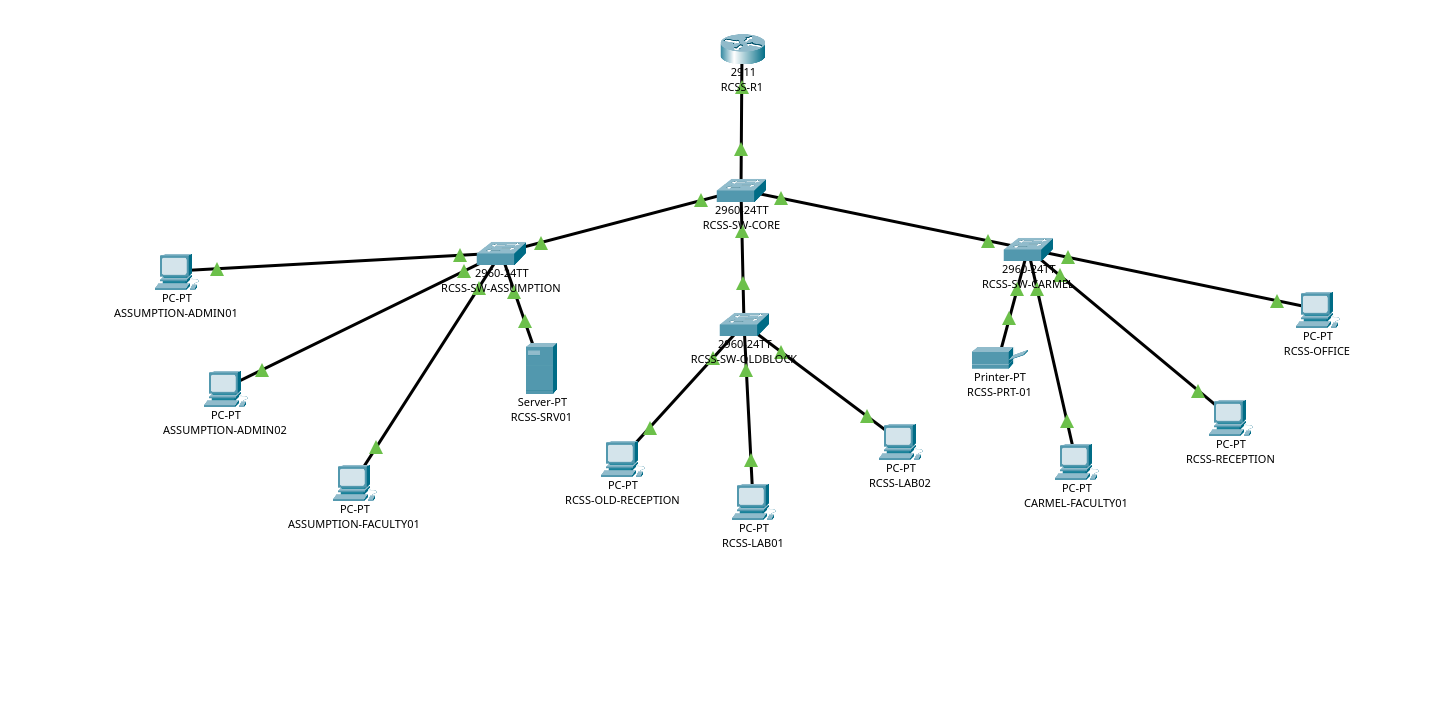
\includegraphics[width=0.97\linewidth]{screenshots/01_full_topology.png}
\caption{Complete RCSS campus network topology in Cisco Packet Tracer. The router
\texttt{RCSS-R1} connects to the core switch \texttt{RCSS-SW-CORE}, which in turn connects
to the three building switches and, through them, to the eleven end devices.}
\label{fig:topology}
\end{figure}
\end{landscape}

\noindent
The physical layout of the campus does not determine VLAN membership. The printer
\texttt{RCSS-PRT-01} and the two office devices \texttt{RCSS-RECEPTION} and
\texttt{RCSS-OFFICE} are physically connected to the Carmel switch, but their access
ports are configured for VLAN 10, so they belong to the Assumption broadcast domain
alongside the Assumption building hosts. Conversely, the server \texttt{RCSS-SRV01} is
plugged into the Assumption switch but is assigned to the server VLAN 40. Physical
cabling decides reachability; switch-port configuration decides the logical domain.

\begin{table}[H]
\centering
\small
\caption{Core uplinks and the cables that implement them}
\label{tab:uplinks}
\begin{tabular}{@{}L{0.22\textwidth} L{0.12\textwidth} L{0.22\textwidth} L{0.12\textwidth} L{0.16\textwidth}@{}}
\toprule
\textbf{Device A} & \textbf{Port A} & \textbf{Device B} & \textbf{Port B} & \textbf{Purpose} \\
\midrule
\texttt{RCSS-R1}      & \texttt{Gi0/0} & \texttt{RCSS-SW-CORE}      & \texttt{Gi0/1} & Router-on-a-stick trunk \\
\texttt{RCSS-SW-CORE} & \texttt{Gi0/2} & \texttt{RCSS-SW-ASSUMPTION} & \texttt{Gi0/1} & Building uplink \\
\texttt{RCSS-SW-CORE} & \texttt{Fa0/1} & \texttt{RCSS-SW-CARMEL}     & \texttt{Gi0/1} & Building uplink \\
\texttt{RCSS-SW-CORE} & \texttt{Fa0/2} & \texttt{RCSS-SW-OLDBLOCK}   & \texttt{Gi0/1} & Building uplink \\
\bottomrule
\end{tabular}
\end{table}

\noindent
Two of the building uplinks terminate on Fast Ethernet ports of the core switch
(\texttt{Fa0/1} to Carmel and \texttt{Fa0/2} to Old Block). The physical link speed of
those two building paths is therefore limited to 100 Mbit/s by the Fast Ethernet
interfaces, whereas the router link and the Assumption uplink run over Gigabit
Ethernet.

\figref{fig:topology-assumption} and \figref{fig:topology-carmel} enlarge the two halves
of the same topology so that the port-level cabling can be read on paper.

\begin{figure}[H]
\centering
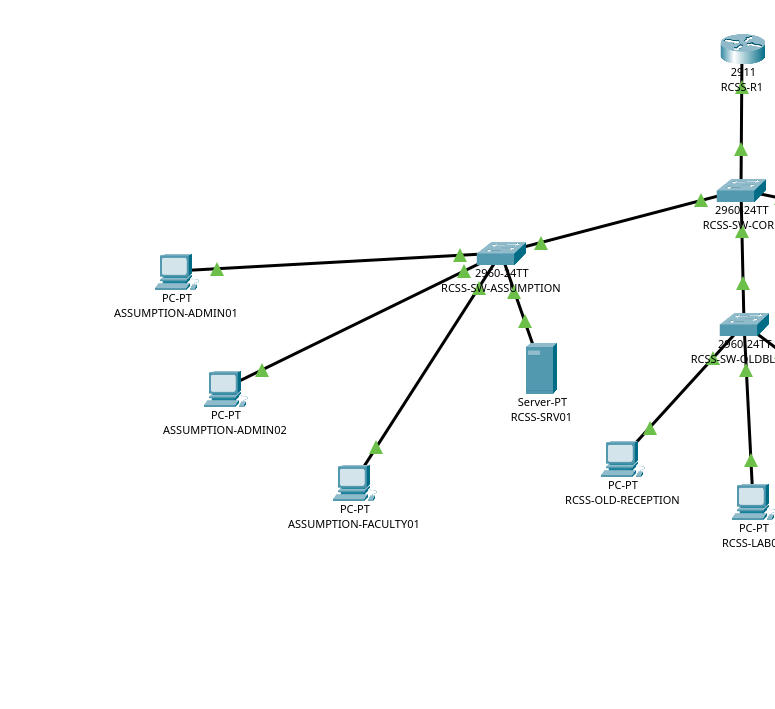
\includegraphics[width=0.92\textwidth]{screenshots/09_topology_assumption_detail.png}
\caption{Enlarged left half of the topology: the Assumption block with
\texttt{ASSUMPTION-ADMIN01}, \texttt{ASSUMPTION-ADMIN02}, \texttt{ASSUMPTION-FACULTY01}
and the server \texttt{RCSS-SRV01}, together with the core switch and the router.}
\label{fig:topology-assumption}
\end{figure}

\begin{figure}[H]
\centering
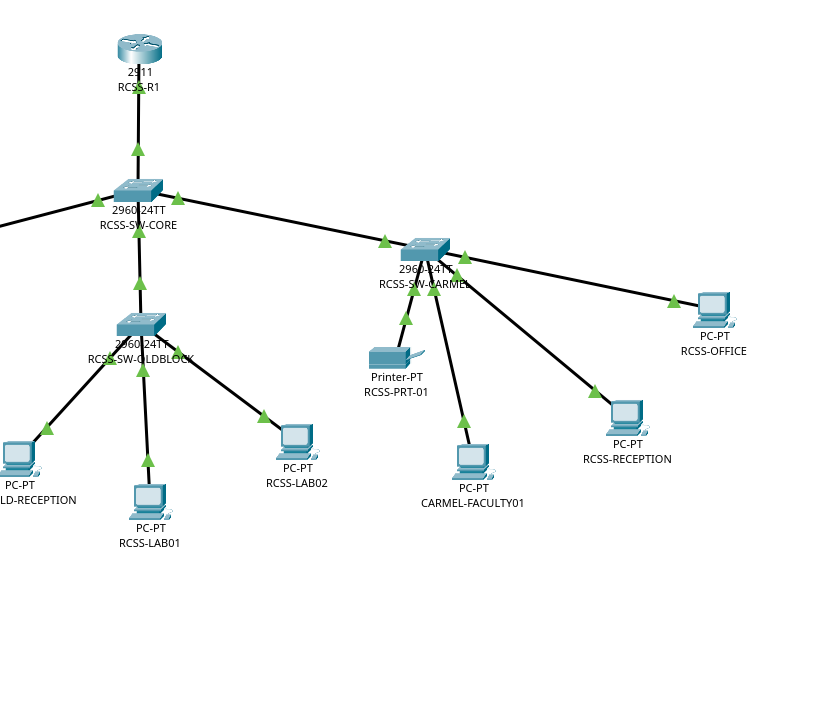
\includegraphics[width=0.92\textwidth]{screenshots/10_topology_carmel_oldblock_detail.png}
\caption{Enlarged right half of the topology: the Carmel block (printer, faculty PC,
reception and office devices), the Old Block laboratory (two lab PCs and the old
reception device) and their uplinks to the core switch.}
\label{fig:topology-carmel}
\end{figure}

% ==========================================================================
% 6. LOGICAL DESIGN AND VLAN PLAN
% ==========================================================================
\section{Logical Design and VLAN Plan}
\label{sec:logical}

\noindent
The campus is segmented into four VLANs. The VLAN ID is the authoritative identifier
that must match across every device; the VLAN name is a human-readable label that is
free to differ between switches.

\begin{table}[H]
\centering
\small
\caption{VLAN plan with the corresponding IP subnets and gateways}
\label{tab:vlans}
\begin{tabular}{@{}C{0.07\textwidth} L{0.19\textwidth} L{0.25\textwidth} L{0.19\textwidth} L{0.17\textwidth}@{}}
\toprule
\textbf{VLAN} & \textbf{Name on core} & \textbf{Purpose} & \textbf{Subnet} & \textbf{Gateway} \\
\midrule
10 & \texttt{ASSUMPTION-BLOCK} & Assumption building and the shared devices that are
                                assigned to it & \texttt{192.168.10.0/24} & \texttt{192.168.10.1} \\
20 & \texttt{CARMEL-BLOCK}    & Carmel faculty workstations &
                                \texttt{192.168.20.0/24} & \texttt{192.168.20.1} \\
30 & \texttt{OLDBLOCK\_LAB}  & Old Block laboratory and old reception &
                                \texttt{192.168.30.0/24} & \texttt{192.168.30.1} \\
40 & \texttt{SERVERS}         & Server network & \texttt{192.168.40.0/24} & \texttt{192.168.40.1} \\
\bottomrule
\end{tabular}
\end{table}

\subsection{Endpoint to VLAN assignment}

\begin{table}[H]
\centering
\small
\caption{Endpoint devices, their access ports and their assigned VLAN}
\label{tab:endpoints}
\begin{tabular}{@{}L{0.30\textwidth} L{0.17\textwidth} L{0.19\textwidth} L{0.22\textwidth}@{}}
\toprule
\textbf{Device} & \textbf{Access switch / port} & \textbf{VLAN ID} & \textbf{Addressing} \\
\midrule
\texttt{ASSUMPTION-ADMIN01}      & Assumption \texttt{Fa0/1} & 10 & DHCP \\
\texttt{ASSUMPTION-ADMIN02}      & Assumption \texttt{Fa0/2} & 10 & DHCP \\
\texttt{RCSS-SRV01}              & Assumption \texttt{Fa0/3} & 40 & Static \texttt{192.168.40.2} \\
\texttt{ASSUMPTION-FACULTY01}    & Assumption \texttt{Fa0/4} & 10 & DHCP \\
\texttt{RCSS-PRT-01}             & Carmel \texttt{Fa0/1}    & 10 & DHCP \\
\texttt{CARMEL-FACULTY01}        & Carmel \texttt{Fa0/2}    & 20 & DHCP \\
\texttt{RCSS-RECEPTION}          & Carmel \texttt{Fa0/3}    & 10 & DHCP \\
\texttt{RCSS-OFFICE}             & Carmel \texttt{Fa0/4}    & 10 & DHCP \\
\texttt{RCSS-LAB01}              & Old Block \texttt{Fa0/1} & 30 & DHCP \\
\texttt{RCSS-LAB02}              & Old Block \texttt{Fa0/2} & 30 & DHCP \\
\texttt{RCSS-OLD-RECEPTION}      & Old Block \texttt{Fa0/3} & 30 & DHCP \\
\bottomrule
\end{tabular}
\end{table}

\noindent
The names used for a VLAN may differ between switches without affecting forwarding. The
core names VLAN 30 \texttt{OLDBLOCK\_LAB}, whereas the Old Block switch names the same
VLAN \texttt{OLDBLOCK-LAB}. As long as the numeric ID 30 is identical on both sides of
the trunk and the trunk carries that VLAN, frames are classified into the same VLAN at
both ends regardless of the label.

\subsection{Router interface state}

\figref{fig:router-if} is the \texttt{show ip interface brief} output of
\texttt{RCSS-R1}. The physical \texttt{GigabitEthernet0/0} carries no IP address of its
own, which is correct for router-on-a-stick, and its four tagged subinterfaces are all
\textit{up/up} with the gateway address of their own subnet. The remaining interfaces
(\texttt{GigabitEthernet0/1}, \texttt{GigabitEthernet0/2} and \texttt{Vlan1}) are
unassigned and administratively down, which simply means they were never used.

\begin{figure}[H]
\centering
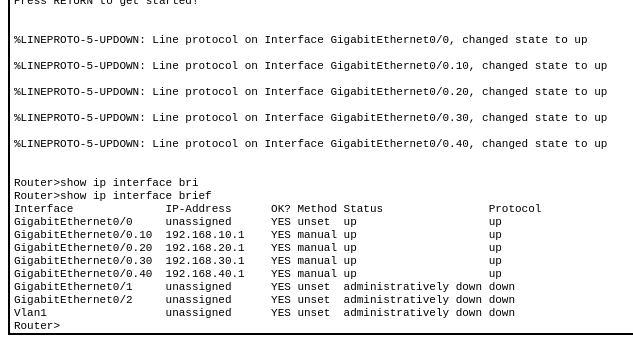
\includegraphics[width=0.95\textwidth]{screenshots/02_router_ip_interface_brief.png}
\caption{\texttt{show ip interface brief} on \texttt{RCSS-R1}. The four subinterfaces
\texttt{Gi0/0.10} to \texttt{Gi0/0.40} are up/up with the gateway addresses of VLANs 10,
20, 30 and 40; the physical \texttt{Gi0/0} is up/up and carries the trunk.}
\label{fig:router-if}
\end{figure}

\subsection{Core switch VLANs and trunks}

\figref{fig:core-vlan} is the \texttt{show vlan brief} output of the core switch. The
four VLANs 10, 20, 30 and 40 exist and are active, together with the VLAN 1 default and
the four default VLANs 1002--1005 that Cisco keeps on every switch. The core switch has
no access ports, so no endpoint appears in the Ports column: all four of its uplinks
(\texttt{Gi0/1}, \texttt{Gi0/2}, \texttt{Fa0/1}, \texttt{Fa0/2}) are trunks, and
Packet Tracer omits trunk ports from the VLAN table.

\begin{figure}[H]
\centering
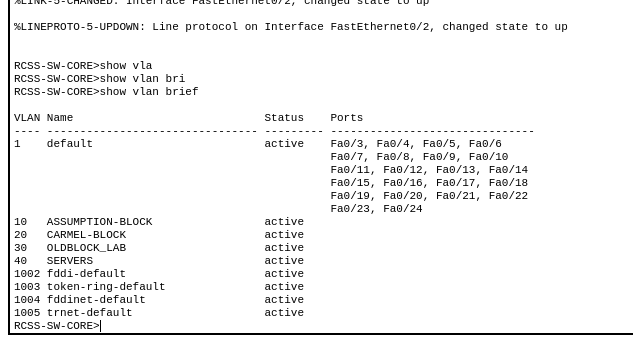
\includegraphics[width=0.95\textwidth]{screenshots/03_core_vlan_brief.png}
\caption{\texttt{show vlan brief} on \texttt{RCSS-SW-CORE}. VLANs 10, 20, 30 and 40 are
active; no access ports are listed because every core port is a trunk.}
\label{fig:core-vlan}
\end{figure}

\figref{fig:core-trunk} is the \texttt{show interfaces trunk} output of the same
switch. All four ports report \texttt{802.1q} encapsulation and status \texttt{trunking},
with native VLAN 1 and the full 1--1005 range allowed. The active VLAN list and the
spanning-tree forwarding list both contain exactly \texttt{1, 10, 20, 30, 40}, which
confirms that all four VLANs are permitted and forwarding across every core trunk.

\begin{figure}[H]
\centering
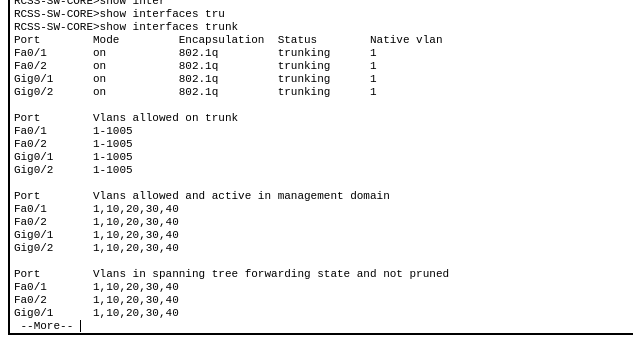
\includegraphics[width=0.95\textwidth]{screenshots/04_core_interfaces_trunk.png}
\caption{\texttt{show interfaces trunk} on \texttt{RCSS-SW-CORE}. Ports \texttt{Fa0/1},
\texttt{Fa0/2}, \texttt{Gi0/1} and \texttt{Gi0/2} are all 802.1Q trunks carrying VLANs
1, 10, 20, 30 and 40.}
\label{fig:core-trunk}
\end{figure}

\subsection{Building switch access ports}

\figref{fig:assumption-vlan} shows the Assumption switch. VLAN 10 (named
\texttt{ASSUMPTION-BLOCK}) holds the access ports \texttt{Fa0/1}, \texttt{Fa0/2} and
\texttt{Fa0/4}, which are the two admin PCs and the Assumption faculty PC. VLAN 40
(\texttt{SERVERS}) holds \texttt{Fa0/3}, the port of the server, so the server's
traffic is carried as tagged VLAN 40 over the uplink to the core.

\begin{figure}[H]
\centering
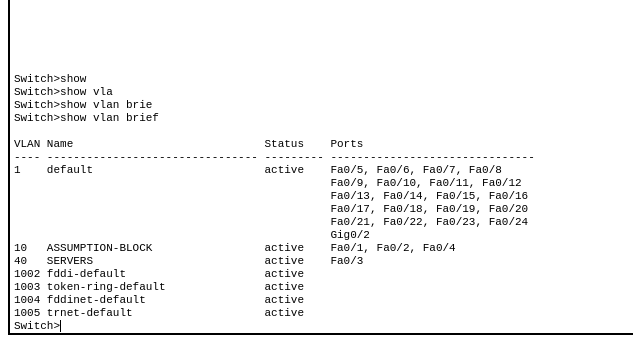
\includegraphics[width=0.95\textwidth]{screenshots/05_assumption_vlan_brief.png}
\caption{\texttt{show vlan brief} on \texttt{RCSS-SW-ASSUMPTION}. VLAN 10 carries the
access ports Fa0/1, Fa0/2 and Fa0/4; VLAN 40 carries Fa0/3, the server port.}
\label{fig:assumption-vlan}
\end{figure}

\figref{fig:carmel-vlan} shows the Carmel switch. VLAN 10 (\texttt{ASSUMPTION-BLOCK})
carries the printer, reception and office ports \texttt{Fa0/1}, \texttt{Fa0/3} and
\texttt{Fa0/4}, while VLAN 20 (\texttt{CARMEL-BLOCK}) carries only \texttt{Fa0/2}, the
Carmel faculty PC. This is the clearest illustration that VLAN membership follows the
port configuration and not the building: three of the four devices plugged into the
Carmel switch belong to the Assumption broadcast domain.

\begin{figure}[H]
\centering
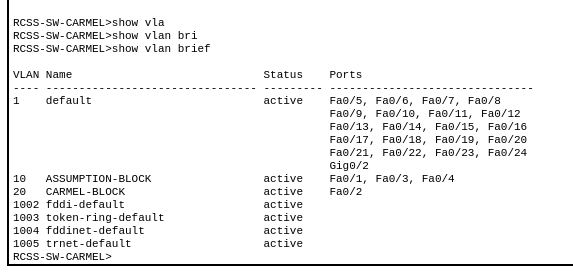
\includegraphics[width=0.95\textwidth]{screenshots/06_carmel_vlan_brief.png}
\caption{\texttt{show vlan brief} on \texttt{RCSS-SW-CARMEL}. VLAN 10 carries Fa0/1,
Fa0/3 and Fa0/4; VLAN 20 carries Fa0/2. The port \texttt{Gi0/2} is listed under the
default VLAN 1 and is unused (see Section~\ref{sec:discrepancies}).}
\label{fig:carmel-vlan}
\end{figure}

\figref{fig:oldblock-vlan} is the corresponding output for the Old Block switch. The
switch carries only one network VLAN, VLAN 30, named \texttt{OLDBLOCK-LAB} here, and
all three of its endpoint ports \texttt{Fa0/1}, \texttt{Fa0/2} and \texttt{Fa0/3} sit in
that VLAN. The name differs from the core switch's \texttt{OLDBLOCK\_LAB}, which is
irrelevant as long as the numeric ID matches on both sides of the trunk.

\begin{figure}[H]
\centering
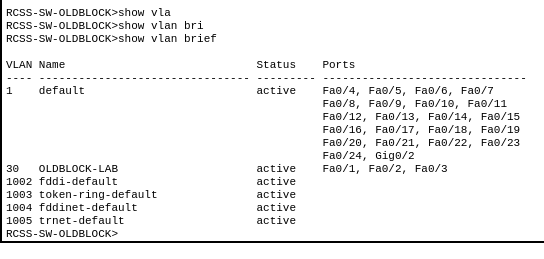
\includegraphics[width=0.95\textwidth]{screenshots/11_oldblock_vlan_brief.png}
\caption{\texttt{show vlan brief} on \texttt{RCSS-SW-OLDBLOCK}. VLAN 30
(\texttt{OLDBLOCK-LAB}) carries the three access ports Fa0/1, Fa0/2 and Fa0/3.}
\label{fig:oldblock-vlan}
\end{figure}

\subsection{Building switch uplinks}

\figref{fig:assumption-trunk}, \figref{fig:carmel-trunk} and \figref{fig:oldblock-trunk}
are the \texttt{show interfaces trunk} outputs of the three building switches. In each
case the uplink \texttt{Gi0/1} reports 802.1Q encapsulation and status
\texttt{trunking}, with the native VLAN 1 and the full range 1--1005 allowed. The
active VLAN list matches the VLANs actually used in that building: VLANs 1, 10 and 40
on the Assumption switch, VLANs 1, 10 and 20 on the Carmel switch, and VLANs 1 and 30
on the Old Block switch. Only the VLANs that exist on the building switch are carried
over its uplink, which keeps the trunks efficient.

\begin{figure}[H]
\centering
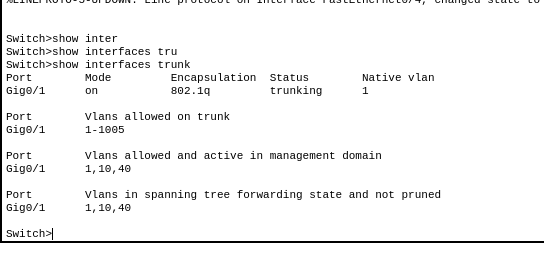
\includegraphics[width=0.95\textwidth]{screenshots/12_assumption_trunk.png}
\caption{\texttt{show interfaces trunk} on \texttt{RCSS-SW-ASSUMPTION}. The uplink
\texttt{Gi0/1} is trunking and carries VLANs 1, 10 and 40.}
\label{fig:assumption-trunk}
\end{figure}

\begin{figure}[H]
\centering
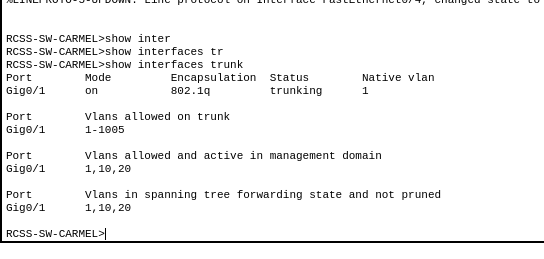
\includegraphics[width=0.95\textwidth]{screenshots/13_carmel_trunk.png}
\caption{\texttt{show interfaces trunk} on \texttt{RCSS-SW-CARMEL}. The uplink
\texttt{Gi0/1} is trunking and carries VLANs 1, 10 and 20. This confirms that
\texttt{Gi0/1}, and not \texttt{Gi0/2}, is the active Carmel uplink.}
\label{fig:carmel-trunk}
\end{figure}

\begin{figure}[H]
\centering
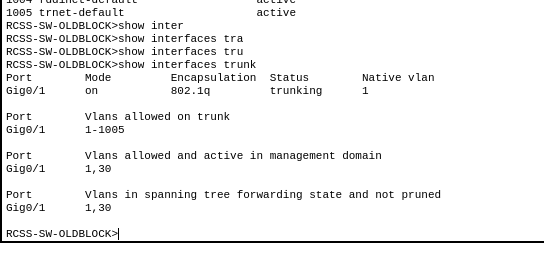
\includegraphics[width=0.95\textwidth]{screenshots/14_oldblock_trunk.png}
\caption{\texttt{show interfaces trunk} on \texttt{RCSS-SW-OLDBLOCK}. The uplink
\texttt{Gi0/1} is trunking and carries VLANs 1 and 30.}
\label{fig:oldblock-trunk}
\end{figure}

% ==========================================================================
% 7. SUBNETTING CALCULATIONS
% ==========================================================================
\section{Subnetting Calculations}
\label{sec:subnet}

\noindent
Every VLAN in this design uses the mask \texttt{255.255.255.0}, which is a prefix of
/24. The derivation is as follows.

\begin{align*}
  \text{Address length}      &= 32\ \text{bits} \\
  \text{Network bits}        &= 24 \\
  \text{Host bits}           &= 32 - 24 = 8 \\
  \text{Total addresses}     &= 2^{8} = 256 \\
  \text{Usable host addresses} &= 256 - 2 = 254
\end{align*}

\noindent
The two addresses that are removed from the usable count are the network address (the
all-zero host part) and the broadcast address (the all-one host part). Neither may be
assigned to an ordinary host: the network address identifies the subnet itself, and the
broadcast address is used for directed broadcasts to every host in the subnet.

\begin{table}[H]
\centering
\footnotesize
\caption{Address arithmetic for the four /24 subnets}
\label{tab:subnets}
\begin{tabular}{@{}C{0.08\textwidth} L{0.22\textwidth} L{0.20\textwidth} L{0.20\textwidth} L{0.18\textwidth}@{}}
\toprule
\textbf{VLAN} & \textbf{Network address} & \textbf{First usable} & \textbf{Last usable} & \textbf{Broadcast} \\
\midrule
10 & \texttt{192.168.10.0/24} & \texttt{192.168.10.1} & \texttt{192.168.10.254} & \texttt{192.168.10.255} \\
20 & \texttt{192.168.20.0/24} & \texttt{192.168.20.1} & \texttt{192.168.20.254} & \texttt{192.168.20.255} \\
30 & \texttt{192.168.30.0/24} & \texttt{192.168.30.1} & \texttt{192.168.30.254} & \texttt{192.168.30.255} \\
40 & \texttt{192.168.40.0/24} & \texttt{192.168.40.1} & \texttt{192.168.40.254} & \texttt{192.168.40.255} \\
\bottomrule
\end{tabular}
\end{table}

\noindent
In each of these subnets the fourth octet \texttt{0} is the network address, the fourth
octet \texttt{255} is the broadcast address, and the fourth octet \texttt{1} is assigned
to the router's subinterface for that VLAN, which makes it the default gateway of the
subnet. The choice of the 192.168.10.0, 192.168.20.0, 192.168.30.0 and 192.168.40.0
subnets keeps the first three octets identical, which makes the router's connected
routes easy to recognise in the routing table.

% ==========================================================================
% 8. IP ADDRESSING AND DHCP PLAN
% ==========================================================================
\section{IP Addressing and DHCP Plan}
\label{sec:ipdhcp}

\subsection{Client addressing}

\noindent
The router runs four DHCP pools, one per VLAN. In each subnet the range
.\textit{x}.1 to .\textit{x}.20 is excluded so that the gateway and a block of
addresses for static or future use are protected from automatic allocation. The
resulting scope is .\textit{x}.21 to .\textit{x}.254.

\begin{table}[H]
\centering
\footnotesize
\caption{DHCP scopes after the reserved low range}
\label{tab:dhcp}
\begin{tabular}{@{}C{0.06\textwidth} L{0.18\textwidth} L{0.17\textwidth} L{0.27\textwidth} L{0.26\textwidth}@{}}
\toprule
\textbf{VLAN} & \textbf{Subnet} & \textbf{Gateway} & \textbf{Excluded range} & \textbf{Available DHCP range} \\
\midrule
10 & \texttt{192.168.10.0/24} & \texttt{192.168.10.1} & \texttt{192.168.10.1} to \texttt{192.168.10.20} & \texttt{192.168.10.21} to \texttt{192.168.10.254} \\
20 & \texttt{192.168.20.0/24} & \texttt{192.168.20.1} & \texttt{192.168.20.1} to \texttt{192.168.20.20} & \texttt{192.168.20.21} to \texttt{192.168.20.254} \\
30 & \texttt{192.168.30.0/24} & \texttt{192.168.30.1} & \texttt{192.168.30.1} to \texttt{192.168.30.20} & \texttt{192.168.30.21} to \texttt{192.168.30.254} \\
40 & \texttt{192.168.40.0/24} & \texttt{192.168.40.1} & \texttt{192.168.40.1} to \texttt{192.168.40.20} & \texttt{192.168.40.21} to \texttt{192.168.40.254} \\
\bottomrule
\end{tabular}
\end{table}

\noindent
These are the \emph{available} ranges after the exclusions. The address that a given
client finally receives depends on the order of the requests and on which addresses are
already in use; the exclusions only guarantee that an address in the reserved block is
never handed out.

\subsection{Static addressing of the server}

\noindent
The campus server \texttt{RCSS-SRV01} is configured statically so that other devices
can reach it at a predictable address:

\begin{table}[H]
\centering
\small
\caption{Static configuration of \texttt{RCSS-SRV01}}
\begin{tabular}{@{}L{0.4\textwidth} L{0.45\textwidth}@{}}
\toprule
\textbf{Field} & \textbf{Value} \\
\midrule
IPv4 address      & \texttt{192.168.40.2} \\
Subnet mask       & \texttt{255.255.255.0} \\
Default gateway   & \texttt{192.168.40.1} \\
DNS server        & Not configured (left blank) \\
\bottomrule
\end{tabular}
\end{table}

\noindent
The address 192.168.40.2 lies inside the excluded range 192.168.40.1--192.168.40.20 of
the server pool, so the DHCP service can never lease it to another device. The
\texttt{show ip dhcp pool} output in \figref{fig:dhcp} confirms this from the server
side: the \texttt{SERVERS} pool reports zero leased addresses.

\subsection{DHCP pool state}

\figref{fig:dhcp} is the \texttt{show ip dhcp pool} output of the router. The four
pools \texttt{ASSUMPTION}, \texttt{CARMEL}, \texttt{OLDBLOCK} and \texttt{SERVERS} all
exist, each with a total of 254 addresses and four excluded addresses. The lease
counters are consistent with the endpoint plan of
Table~\ref{tab:endpoints}: six leases in the Assumption pool (the two admin PCs, the
Assumption faculty PC, the printer, the reception PC and the office PC), one lease in
the Carmel pool (the Carmel faculty PC), three leases in the Old Block pool (the two lab
PCs and the old reception PC) and no lease in the server pool.

\begin{figure}[H]
\centering
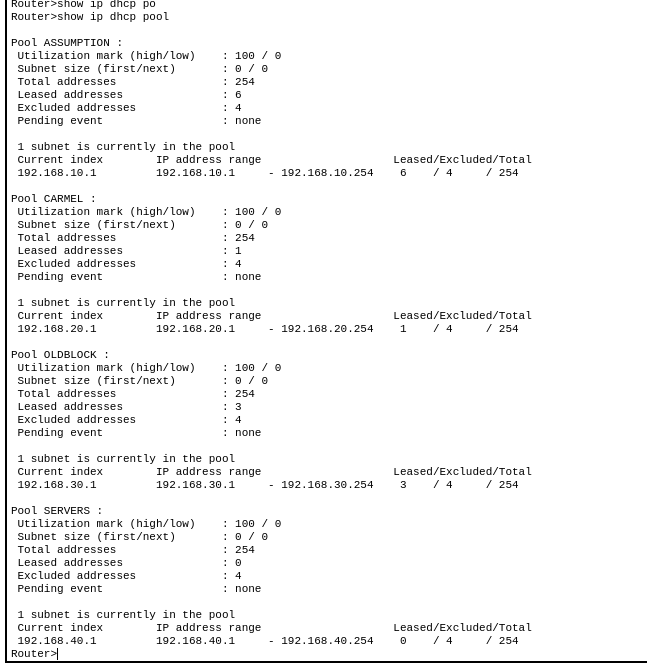
\includegraphics[width=0.86\textwidth]{screenshots/07_router_dhcp_pool.png}
\caption{\texttt{show ip dhcp pool} on \texttt{RCSS-R1}. Four pools are defined; six
clients are leased in the Assumption pool, one in Carmel, three in Old Block and none
in the server pool, which is consistent with the static server address.}
\label{fig:dhcp}
\end{figure}

\figref{fig:dhcp-bindings} is the \texttt{show ip dhcp binding} table. It lists the
address actually leased to each client together with its hardware (MAC) address. Six
leases exist in the VLAN 10 subnet (192.168.10.21, .22, .23, .24, .25 and .26), one in
the VLAN 20 subnet (192.168.20.21) and two in the VLAN 30 subnet (192.168.30.22 and
192.168.30.23). Two properties of this table are worth noting. First, the lowest
leased address in every subnet is .21, which confirms that the excluded range
.\textit{x}.1 to .\textit{x}.20 is honoured by the service. Second, no lease exists in
the server subnet, which confirms that the statically addressed server is outside the
pool.

\begin{figure}[H]
\centering
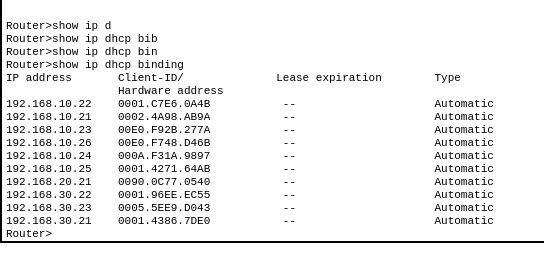
\includegraphics[width=0.95\textwidth]{screenshots/15_dhcp_bindings.png}
\caption{\texttt{show ip dhcp binding} on \texttt{RCSS-R1}. Six leases in the VLAN 10
subnet, one in VLAN 20 and two in VLAN 30; every lease starts at .21 or above, and no
lease exists in the server subnet.}
\label{fig:dhcp-bindings}
\end{figure}

% ==========================================================================
% 9. CONFIGURATION PROCEDURE
% ==========================================================================
\section{Configuration Procedure}
\label{sec:config}

\noindent
The network was built in the following order. Each stage depends on the previous one,
because a trunk must carry a VLAN before a device in that VLAN can reach its gateway.

\subsection{Core switch}

\noindent
The four VLANs are created and named on the core switch, and every core port that must
carry more than one VLAN is converted into a trunk:

\begin{lstlisting}[caption={Core switch \texttt{RCSS-SW-CORE}}]
enable
configure terminal
no ip domain-lookup
vlan 10
 name ASSUMPTION-BLOCK
exit
vlan 20
 name CARMEL-BLOCK
exit
vlan 30
 name OLDBLOCK_LAB
exit
vlan 40
 name SERVERS
exit
interface gigabitEthernet 0/1
 switchport mode trunk
exit
interface gigabitEthernet 0/2
 switchport mode trunk
exit
interface fastEthernet 0/1
 switchport mode trunk
exit
interface fastEthernet 0/2
 switchport mode trunk
exit
end
\end{lstlisting}

\subsection{Building switches}

\noindent
The same procedure is repeated on each building switch: create the VLANs that the
building actually needs, set the uplink to trunk mode, and assign each endpoint port
to its access VLAN. On the Assumption switch, for example:

\begin{lstlisting}[caption={Assumption switch \texttt{RCSS-SW-ASSUMPTION}}]
vlan 10
 name ASSUMPTION-BLOCK
exit
vlan 40
 name SERVERS
exit
interface gigabitEthernet 0/1
 switchport mode trunk
exit
interface range fastEthernet 0/1 - 2
 switchport access vlan 10
exit
interface fastEthernet 0/3
 switchport access vlan 40
exit
interface fastEthernet 0/4
 switchport access vlan 10
exit
\end{lstlisting}

\noindent
The Carmel switch creates VLANs 10 and 20 and places the printer, reception and office
ports in VLAN 10 and the faculty port in VLAN 20. The Old Block switch creates only
VLAN 30, named \texttt{OLDBLOCK-LAB}, and puts its three endpoint ports into it. The
different VLAN name on the Old Block switch is harmless, because only the numeric VLAN
ID has to match across the trunk.

\subsection{Router and 802.1Q subinterfaces}

\noindent
The router interface is enabled and the four subinterfaces are created. The physical
interface deliberately keeps \texttt{no ip address} so that the tagged subinterfaces
alone hold the gateway addresses:

\begin{lstlisting}[caption={Router \texttt{RCSS-R1} --- router-on-a-stick}]
interface gigabitEthernet 0/0
 no ip address
 no shutdown
exit
interface gigabitEthernet 0/0.10
 encapsulation dot1Q 10
 ip address 192.168.10.1 255.255.255.0
exit
interface gigabitEthernet 0/0.20
 encapsulation dot1Q 20
 ip address 192.168.20.1 255.255.255.0
exit
interface gigabitEthernet 0/0.30
 encapsulation dot1Q 30
 ip address 192.168.30.1 255.255.255.0
exit
interface gigabitEthernet 0/0.40
 encapsulation dot1Q 40
 ip address 192.168.40.1 255.255.255.0
exit
\end{lstlisting}

\subsection{DHCP pools and exclusions}

\begin{lstlisting}[caption={DHCP configuration on \texttt{RCSS-R1}}]
ip dhcp excluded-address 192.168.10.1 192.168.10.20
ip dhcp excluded-address 192.168.20.1 192.168.20.20
ip dhcp excluded-address 192.168.30.1 192.168.30.20
ip dhcp excluded-address 192.168.40.1 192.168.40.20
ip dhcp pool ASSUMPTION
 network 192.168.10.0 255.255.255.0
 default-router 192.168.10.1
exit
ip dhcp pool CARMEL
 network 192.168.20.0 255.255.255.0
 default-router 192.168.20.1
exit
ip dhcp pool OLDBLOCK
 network 192.168.30.0 255.255.255.0
 default-router 192.168.30.1
exit
ip dhcp pool SERVERS
 network 192.168.40.0 255.255.255.0
 default-router 192.168.40.1
exit
\end{lstlisting}

\subsection{End devices, verification and save}

\noindent
The server receives its static configuration through the Desktop tab of
\texttt{RCSS-SRV01}; every other PC and the printer are switched to DHCP on their IP
Configuration page. The state is then verified with \texttt{show vlan brief},
\texttt{show interfaces trunk}, \texttt{show ip interface brief},
\texttt{show ip dhcp pool}, \texttt{show ip dhcp binding}, \texttt{show ip route} and
ICMP pings, and finally saved on every device with
\texttt{copy running-config startup-config} before the Packet Tracer project itself is
saved.

% ==========================================================================
% 10. VERIFICATION AND RESULTS
% ==========================================================================
\section{Verification and Results}
\label{sec:verify}

\subsection{What was verified}

\noindent
The following checks were performed and captured:

\begin{itemize}
  \item \textbf{Router interfaces} --- \texttt{show ip interface brief} confirms the four
        subinterfaces are up/up with the correct gateway addresses
        (\figref{fig:router-if}).
  \item \textbf{Core VLANs} --- \texttt{show vlan brief} confirms VLANs 10, 20, 30 and 40
        exist and are active (\figref{fig:core-vlan}).
  \item \textbf{Core trunks} --- \texttt{show interfaces trunk} confirms all four core
        ports are 802.1Q trunks with VLANs 1, 10, 20, 30 and 40 allowed and active
        (\figref{fig:core-trunk}).
  \item \textbf{Access-port membership} --- \texttt{show vlan brief} on the Assumption and
        Carmel switches confirms the endpoint ports are in the intended VLANs
        (\figref{fig:assumption-vlan}, \figref{fig:carmel-vlan}).
  \item \textbf{DHCP pools and leases} --- \texttt{show ip dhcp pool} confirms the four
        pools and the lease counts of Table~\ref{tab:dhcp} (\figref{fig:dhcp}), and
        \texttt{show ip dhcp binding} lists the address and MAC address actually leased
        to each client (\figref{fig:dhcp-bindings}).
  \item \textbf{Building switch uplinks} --- \texttt{show interfaces trunk} on the three
        building switches confirms that each uplink \texttt{Gi0/1} is trunking and
        carries that building's VLANs (\figref{fig:assumption-trunk},
        \figref{fig:carmel-trunk}, \figref{fig:oldblock-trunk}).
  \item \textbf{Old Block access ports} --- \texttt{show vlan brief} confirms that the
        three lab and reception ports sit in VLAN 30 (\figref{fig:oldblock-vlan}).
  \item \textbf{Routing table} --- \texttt{show ip route} confirms the four connected
        subnet routes (\figref{fig:ip-route}).
  \item \textbf{Running configuration} --- \texttt{show running-config} confirms the four
        DHCP exclusions and the four pools (\figref{fig:running-config}).
  \item \textbf{Connectivity} --- an ICMP ping to a client in the VLAN 20 subnet returned
        replies (\figref{fig:ping}).
\end{itemize}

\subsection{Routing table and saved configuration}

\figref{fig:ip-route} is the \texttt{show ip route} output of the router. All four
subnets appear as connected routes, one per subinterface, together with the /32 host
routes that Cisco generates automatically for each gateway address. No default route
is present, which is correct for a campus that has no upstream link, and no static or
dynamic route was configured because the router only needs to route between its own
directly connected networks.

\begin{figure}[H]
\centering
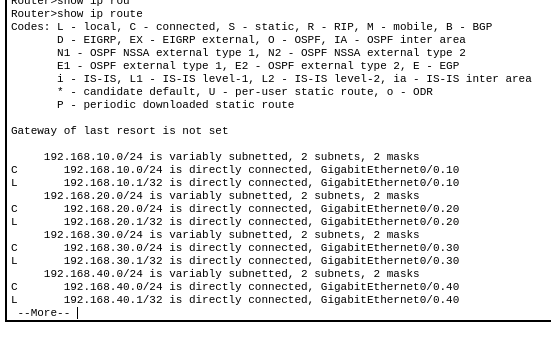
\includegraphics[width=0.95\textwidth]{screenshots/16_ip_route.png}
\caption{\texttt{show ip route} on \texttt{RCSS-R1}. The four campus subnets are
connected through the subinterfaces Gi0/0.10, Gi0/0.20, Gi0/0.30 and Gi0/0.40; there
is no default route.}
\label{fig:ip-route}
\end{figure}

\figref{fig:running-config} shows the DHCP section of the router's
\texttt{show running-config}. The four \texttt{ip dhcp excluded-address} statements
reserve .\textit{x}.1 to .\textit{x}.20 in each subnet, and the four pools carry the
correct network and default-router values. This is the direct confirmation of the
address plan that Section~\ref{sec:discrepancies} discusses.

\begin{figure}[H]
\centering
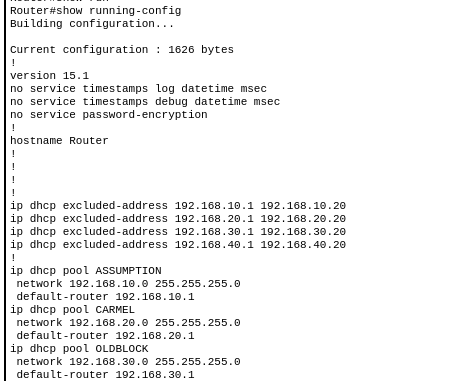
\includegraphics[width=0.9\textwidth]{screenshots/17_running_config_dhcp.png}
\caption{DHCP section of \texttt{show running-config} on \texttt{RCSS-R1}. The excluded
ranges .\textit{x}.1 to .\textit{x}.20 and the four pools with their networks and
default routers are present in the running configuration.}
\label{fig:running-config}
\end{figure}

\subsection{Connectivity test}

\figref{fig:ping} is the only ping capture in the evidence set. Four echo requests were
sent to 192.168.20.21 and three replies were received, so the recorded result is
\textbf{4 sent, 3 received, 1 lost (25\% loss)}. The first request timed out while the
address resolution for the destination was still being completed; the three subsequent
requests were answered in about 1\,ms with a round-trip time of 0\,ms as the minimum,
average and maximum. The destination 192.168.20.21 is the first address above the
reserved range of the Carmel pool, which is consistent with a DHCP lease held by
\texttt{CARMEL-FACULTY01}.

\begin{figure}[H]
\centering
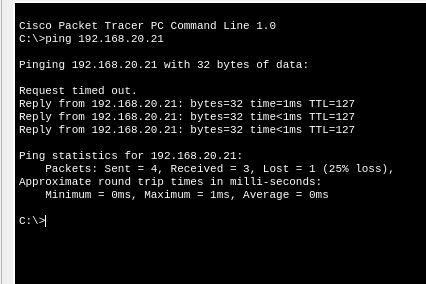
\includegraphics[width=0.62\textwidth]{screenshots/08_inter_vlan_ping_test.png}
\caption{ICMP ping to 192.168.20.21. Four requests were sent and three replies were
received (25\% loss); the first request timed out during address resolution.}
\label{fig:ping}
\end{figure}

\subsection{Test results table}

\begin{table}[H]
\centering
\small
\caption{Connectivity tests and the evidence available for each of them}
\label{tab:tests}
\begin{tabular}{@{}L{0.19\textwidth} L{0.21\textwidth} L{0.22\textwidth} L{0.28\textwidth}@{}}
\toprule
\textbf{Test} & \textbf{Source} & \textbf{Destination} & \textbf{Observed result} \\
\midrule
Gateway test       & \texttt{ASSUMPTION-ADMIN01} & \texttt{192.168.10.1} & Not captured \\
Gateway test       & \texttt{RCSS-SRV01}         & \texttt{192.168.40.1} & Not captured \\
Inter-VLAN test    & \texttt{RCSS-SRV01}         & Admin01's address  & Not captured \\
Cross-building test & \texttt{ASSUMPTION-ADMIN01} & Carmel Faculty01's address (\texttt{192.168.20.21}) & Ping to \texttt{192.168.20.21}: 4 sent, 3 received, 1 lost (25\% loss) \\
Inter-VLAN test    & \texttt{RCSS-LAB01}         & \texttt{192.168.40.2} & Not captured \\
\bottomrule
\end{tabular}
\end{table}

\noindent
A gateway ping proves that the router interface of a VLAN is reachable from an
endpoint. A ping between two endpoints in different VLANs proves more, because the
traffic has to be tagged, carried over a trunk, de-tagged by a router subinterface and
routed into the destination subnet. The single capture in
\figref{fig:ping} is a routed test, because 192.168.20.21 and the source of the ping
are not on the same subnet in the address plan, and it did receive replies. The four
tests that were not captured are listed again in Appendix~\ref{app:evidence}. They
are the two gateway tests and the remaining endpoint-to-endpoint tests; the gateway
reachability they would prove is already implied by the four subinterfaces being up/up
with their gateway addresses, and the routed path itself is demonstrated by the
capture above.

\subsection{Discrepancies between the plan and the captured output}
\label{sec:discrepancies}

\noindent
Two points in the captured output looked like deviations from the written plan when
they were first examined. The additional captures obtained later resolve both of
them, and one smaller point remains open. All three are reported here rather than
being smoothed over.

\begin{enumerate}[label=\textbf{D\arabic*.},leftmargin=2.2em]
  \item \textbf{The DHCP exclusion counters --- resolved.} The intended exclusion in
        every subnet is .\textit{x}.1 to .\textit{x}.20, that is twenty addresses, but
        in \figref{fig:dhcp} Packet Tracer reports \texttt{Excluded addresses : 4} for
        every pool and displays the pool range as .\textit{x}.1 to .\textit{x}.254.
        The \texttt{show running-config} capture in \figref{fig:running-config} shows
        the four \texttt{ip dhcp excluded-address} statements exactly as intended, so
        the configuration is correct and the counter in the pool summary is a display
        artefact of the simulation rather than an error in the configuration. The
        behaviour of the service confirms the same thing: every lease in
        \figref{fig:dhcp-bindings} starts at .21 or above.
  \item \textbf{The Carmel gigabit port \texttt{Gi0/2} --- resolved.} The Carmel switch
        lists \texttt{Gi0/2} in the default VLAN 1 in \figref{fig:carmel-vlan}, while
        the build plan configures \texttt{Gi0/1} as the trunk to the core switch. The
        \texttt{show interfaces trunk} capture in \figref{fig:carmel-trunk} settles the
        point: \texttt{Gi0/1} is the port that reports 802.1Q encapsulation and status
        \texttt{trunking} with VLANs 1, 10 and 20 active. \texttt{Gi0/2} is therefore
        an unused gigabit port left in the default VLAN, and it carries no traffic in
        this design. The same pattern appears on the Old Block switch, whose
        \texttt{Gi0/2} also appears in VLAN 1 while \texttt{Gi0/1} is the trunk
        (\figref{fig:oldblock-trunk}).
  \item \textbf{The TTL value in the captured ping --- still open.} All three replies in
        \figref{fig:ping} show \texttt{TTL=128}. In a strictly modelled path a reply
        that crossed one router would arrive with TTL 127. The destination is now
        identified with certainty, because 192.168.20.21 is the only lease in the
        VLAN 20 subnet and therefore belongs to \texttt{CARMEL-FACULTY01}
        (\figref{fig:dhcp-bindings}), but the source device of the ping is not
        identifiable from the captured window, so the capture cannot be attributed to
        a specific named source with certainty. The result is reported as it stands.
  \item \textbf{Old Block lease count.} The pool summary in \figref{fig:dhcp} reports
        three leased addresses in the Old Block pool, while the binding table in
        \figref{fig:dhcp-bindings} lists only two VLAN 30 leases,
        192.168.30.22 and 192.168.30.23, although three endpoints (the two lab PCs and
        the old reception PC) are configured in VLAN 30. One of the three VLAN 30
        clients therefore holds no entry in the binding table at the moment the
        capture was taken. This is a minor bookkeeping difference in the simulation
        and it does not affect the inter-VLAN results, but it is noted so that the
        two outputs are not read as a contradiction.
\end{enumerate}

% ==========================================================================
% 11. DISCUSSION
% ==========================================================================
\section{Discussion}

\noindent
\textbf{VLANs as logical segmentation.} The four VLANs divide the campus into four
independent Layer 2 broadcast domains. A device in VLAN 10 sends a broadcast only to
the other VLAN 10 members, even though the physical switches are shared. The VLAN
table of the core switch and the access-port assignments of the building switches show
that this segmentation is in place and that the four client groups are kept apart.

\noindent
\textbf{Default gateways for different subnets.} Every VLAN is a separate IP subnet,
so an endpoint that needs to reach a different subnet must hand the packet to a
default gateway. The router's four subinterfaces provide exactly one such gateway per
subnet, and the \texttt{show ip interface brief} output confirms that all four are
operational.

\noindent
\textbf{IEEE 802.1Q tagging.} The core switch carries four VLANs over four trunks, and
the router carries the same four VLANs over a single physical cable. The \texttt{802.1q}
encapsulation shown for every trunk port, together with the active VLAN lists
containing VLANs 10, 20, 30 and 40, shows that the tags are being applied and
interpreted correctly. The build guide's warning that VLAN names may differ between
switches applies here: only the numeric VLAN ID is carried in the tag.

\noindent
\textbf{Why router-on-a-stick.} A single 802.1Q trunk to the router is enough to give
four VLANs a gateway, which keeps the core switch free of layer 3 complexity and saves
router ports. The price is that all inter-VLAN traffic is routed by the same physical
interface, and the four subinterfaces share its bandwidth.

\noindent
\textbf{DHCP exclusions.} Reserving .\textit{x}.1 to .\textit{x}.20 keeps the gateway
address and a block of addresses free for static use or for services added later. The
running configuration confirms the four exclusion statements, and every lease in the
binding table starts at .21 or above, so the reserved block is respected in practice.
The server is the case in point: its static address 192.168.40.2 is inside the reserved
block of the server pool, and the pool and the binding table both show no lease in the
server subnet.

\noindent
\textbf{What the pings do and do not prove.} The successful ping proves that one
specific path worked at the moment it was run. It does not prove that every endpoint
was tested, that every VLAN pair is reachable, or that the network would behave the
same way under real traffic. The 25\% loss in the capture is consistent with the
first request being dropped during address resolution, which is normal behaviour on a
new path, but only one capture exists, so the loss cannot be attributed with certainty.

\noindent
\textbf{Security position.} No access control lists are configured in this project.
Inter-VLAN routing is therefore permitted by default: any host that can reach its own
gateway can reach any other VLAN. The network is a functional logical design, not a
secured one.

% ==========================================================================
% 12. LIMITATIONS AND FUTURE IMPROVEMENTS
% ==========================================================================
\section{Limitations and Future Improvements}
\label{sec:limitations}

\subsection{Limitations}

\begin{itemize}
  \item The network is a Packet Tracer simulation. It has not been deployed on real
        hardware and no physical behaviour, cabling fault or hardware failure has been
        reproduced.
  \item No ACLs and no firewall policies exist, so there is no filtering between
        VLANs.
  \item No DNS service is configured; the server's DNS field is blank and name
        resolution is not available.
  \item No WAN, Internet or upstream link is configured; the router has no default
        route.
  \item There is no redundancy. A single core switch and a single router carry the whole
        campus, and each building has exactly one uplink.
  \item No management VLAN, no SSH access and no monitoring exist; the devices are
        managed through their console.
  \item The Carmel and Old Block uplinks are limited to 100 Mbit/s by the Fast
        Ethernet ports on the core switch.
  \item The evidence set is still incomplete. The endpoint IP configuration pages and
        four of the five planned ping tests were not captured
        (Appendix~\ref{app:evidence}). The router, switch, VLAN, trunk, DHCP and
        routing evidence was captured in full.
\end{itemize}

\subsection{Recommended future improvements}

\noindent
The following are recommendations for a future iteration and are \emph{not} features of
the present design:

\begin{itemize}
  \item \textbf{Inter-VLAN filtering.} ACLs applied to the router subinterfaces would
        allow the VLAN 10 administrative hosts to reach the server VLAN while
        restricting student lab traffic in VLAN 30 to specific destinations.
  \item \textbf{DNS and name services.} A DNS server in the server VLAN, with forwarders
        configured on the router, would let endpoints use host names instead of
        addresses.
  \item \textbf{Redundancy.} A second core switch and a second router, with
        EtherChannel and routing protocol or hot standby, would remove the single
        points of failure.
  \item \textbf{Port security.} Sticky MAC addresses, BPDU guard and DHCP snooping on
        the access ports would limit the damage from an unauthorised device plugged
        into a user port.
  \item \textbf{Management VLAN.} A dedicated VLAN with an SVI on the core switch,
        reached over SSH with AAA and hashed passwords, would keep device management
        off the user VLANs.
  \item \textbf{Monitoring.} Syslog, SNMP polling and bandwidth or link monitoring
        would make failures visible instead of being discovered by a failed ping.
  \item \textbf{Faster server uplink.} Moving the server into the core switch, or
        giving the server VLAN its own Gigabit Ethernet trunk, would remove the
        100 Mbit/s bottleneck on the Carmel and Old Block uplinks.
\end{itemize}

% ==========================================================================
% 13. CONCLUSION
% ==========================================================================
\section{Conclusion}

\noindent
The RCSS campus network was designed and implemented in Cisco Packet Tracer as a
three-building campus served by one Cisco 2911 router and four Cisco 2960 switches.
The four VLANs -- 10 (Assumption), 20 (Carmel), 30 (Old Block lab) and 40 (Servers) --
were created on the core switch, and the router-to-core link together with the three
building uplinks were configured as IEEE 802.1Q trunks, which the captured
\texttt{show interfaces trunk} output confirms. Inter-VLAN routing was implemented
with router-on-a-stick: the physical \texttt{GigabitEthernet0/0} carries no address and
four tagged subinterfaces, \texttt{Gi0/0.10} to \texttt{Gi0/0.40}, provide the gateway
192.168.\textit{x}.1 of each subnet; all four were observed up/up. Four DHCP pools with
a reserved low range were created; the running configuration confirms the four
exclusion statements and the binding table shows every lease starting at .21 or above,
with the server held outside DHCP on the static address 192.168.40.2/24. The routing
table shows the four campus subnets as connected routes through the router's four
subinterfaces. The connectivity evidence that was captured shows a routed ping to
192.168.20.21 answered with three replies out of four requests.

\noindent
The design therefore achieves a working VLAN-segmented campus with automated client
addressing and a statically addressed, reachable server. What it does not yet achieve
is a hardened production network: there are no ACLs, no DNS, no redundancy, no
management plane and no complete test matrix, and the endpoint-level pings still
outstanding should be captured before the design is signed off.

% ==========================================================================
% APPENDICES
% ==========================================================================
\appendix

\section{Router Configuration}
\label{app:router}

\noindent
The router configuration as applied during the build, in the order it was entered.
This is the recorded build configuration; a captured \texttt{show running-config} was
not part of the evidence set, so it has not been diffed against the running state.

\begin{lstlisting}[caption={Full router configuration \texttt{RCSS-R1}}]
enable
configure terminal
no ip domain-lookup
!
interface gigabitEthernet 0/0
 no ip address
 no shutdown
exit
interface gigabitEthernet 0/0.10
 encapsulation dot1Q 10
 ip address 192.168.10.1 255.255.255.0
exit
interface gigabitEthernet 0/0.20
 encapsulation dot1Q 20
 ip address 192.168.20.1 255.255.255.0
exit
interface gigabitEthernet 0/0.30
 encapsulation dot1Q 30
 ip address 192.168.30.1 255.255.255.0
exit
interface gigabitEthernet 0/0.40
 encapsulation dot1Q 40
 ip address 192.168.40.1 255.255.255.0
exit
!
ip dhcp excluded-address 192.168.10.1 192.168.10.20
ip dhcp excluded-address 192.168.20.1 192.168.20.20
ip dhcp excluded-address 192.168.30.1 192.168.30.20
ip dhcp excluded-address 192.168.40.1 192.168.40.20
!
ip dhcp pool ASSUMPTION
 network 192.168.10.0 255.255.255.0
 default-router 192.168.10.1
exit
ip dhcp pool CARMEL
 network 192.168.20.0 255.255.255.0
 default-router 192.168.20.1
exit
ip dhcp pool OLDBLOCK
 network 192.168.30.0 255.255.255.0
 default-router 192.168.30.1
exit
ip dhcp pool SERVERS
 network 192.168.40.0 255.255.255.0
 default-router 192.168.40.1
exit
!
end
copy running-config startup-config
\end{lstlisting}

\section{Switch Configuration}
\label{app:switch}

\noindent
The switch configurations as applied during the build.

\begin{lstlisting}[caption={Core switch \texttt{RCSS-SW-CORE}}]
enable
configure terminal
no ip domain-lookup
vlan 10
 name ASSUMPTION-BLOCK
exit
vlan 20
 name CARMEL-BLOCK
exit
vlan 30
 name OLDBLOCK_LAB
exit
vlan 40
 name SERVERS
exit
interface gigabitEthernet 0/1
 switchport mode trunk
exit
interface gigabitEthernet 0/2
 switchport mode trunk
exit
interface fastEthernet 0/1
 switchport mode trunk
exit
interface fastEthernet 0/2
 switchport mode trunk
exit
end
copy running-config startup-config
\end{lstlisting}

\begin{lstlisting}[caption={Carmel switch \texttt{RCSS-SW-CARMEL}}]
enable
configure terminal
no ip domain-lookup
vlan 10
 name ASSUMPTION-BLOCK
exit
vlan 20
 name CARMEL-BLOCK
exit
interface gigabitEthernet 0/1
 switchport mode trunk
exit
interface fastEthernet 0/1
 switchport access vlan 10
exit
interface fastEthernet 0/2
 switchport access vlan 20
exit
interface range fastEthernet 0/3 - 4
 switchport access vlan 10
exit
end
copy running-config startup-config
\end{lstlisting}

\begin{lstlisting}[caption={Old Block switch \texttt{RCSS-SW-OLDBLOCK}}]
enable
configure terminal
no ip domain-lookup
vlan 30
 name OLDBLOCK-LAB
exit
interface gigabitEthernet 0/1
 switchport mode trunk
exit
interface range fastEthernet 0/1 - 3
 switchport access vlan 30
exit
end
copy running-config startup-config
\end{lstlisting}

\section{Device and Port Map}
\label{app:map}

\small
\begin{longtable}{@{}L{0.24\textwidth} L{0.15\textwidth} L{0.22\textwidth} L{0.29\textwidth}@{}}
\caption{Complete device, port and VLAN map of the campus}\label{tab:map}\\
\toprule
\textbf{Device} & \textbf{Model} & \textbf{Port} & \textbf{Peer / VLAN} \\
\midrule
\endfirsthead
\toprule
\textbf{Device} & \textbf{Model} & \textbf{Port} & \textbf{Peer / VLAN} \\
\midrule
\endhead
\texttt{RCSS-R1}           & Cisco 2911     & \texttt{Gi0/0}    & \texttt{RCSS-SW-CORE} Gi0/1 (trunk) \\
\texttt{RCSS-R1}           & Cisco 2911     & \texttt{Gi0/0.10} & VLAN 10, \texttt{192.168.10.1/24} \\
\texttt{RCSS-R1}           & Cisco 2911     & \texttt{Gi0/0.20} & VLAN 20, \texttt{192.168.20.1/24} \\
\texttt{RCSS-R1}           & Cisco 2911     & \texttt{Gi0/0.30} & VLAN 30, \texttt{192.168.30.1/24} \\
\texttt{RCSS-R1}           & Cisco 2911     & \texttt{Gi0/0.40} & VLAN 40, \texttt{192.168.40.1/24} \\
\texttt{RCSS-SW-CORE}      & Cisco 2960-24TT & \texttt{Gi0/1}    & \texttt{RCSS-R1} Gi0/0 (trunk) \\
\texttt{RCSS-SW-CORE}      & Cisco 2960-24TT & \texttt{Gi0/2}    & \texttt{RCSS-SW-ASSUMPTION} Gi0/1 (trunk) \\
\texttt{RCSS-SW-CORE}      & Cisco 2960-24TT & \texttt{Fa0/1}    & \texttt{RCSS-SW-CARMEL} Gi0/1 (trunk) \\
\texttt{RCSS-SW-CORE}      & Cisco 2960-24TT & \texttt{Fa0/2}    & \texttt{RCSS-SW-OLDBLOCK} Gi0/1 (trunk) \\
\texttt{RCSS-SW-ASSUMPTION} & Cisco 2960    & \texttt{Gi0/1}    & \texttt{RCSS-SW-CORE} Gi0/2 (trunk) \\
\texttt{RCSS-SW-ASSUMPTION} & Cisco 2960    & \texttt{Fa0/1}    & \texttt{ASSUMPTION-ADMIN01}, VLAN 10 \\
\texttt{RCSS-SW-ASSUMPTION} & Cisco 2960    & \texttt{Fa0/2}    & \texttt{ASSUMPTION-ADMIN02}, VLAN 10 \\
\texttt{RCSS-SW-ASSUMPTION} & Cisco 2960    & \texttt{Fa0/3}    & \texttt{RCSS-SRV01}, VLAN 40 \\
\texttt{RCSS-SW-ASSUMPTION} & Cisco 2960    & \texttt{Fa0/4}    & \texttt{ASSUMPTION-FACULTY01}, VLAN 10 \\
\texttt{RCSS-SW-CARMEL}    & Cisco 2960    & \texttt{Gi0/1}    & \texttt{RCSS-SW-CORE} Fa0/1 (trunk) \\
\texttt{RCSS-SW-CARMEL}    & Cisco 2960    & \texttt{Fa0/1}    & \texttt{RCSS-PRT-01}, VLAN 10 \\
\texttt{RCSS-SW-CARMEL}    & Cisco 2960    & \texttt{Fa0/2}    & \texttt{CARMEL-FACULTY01}, VLAN 20 \\
\texttt{RCSS-SW-CARMEL}    & Cisco 2960    & \texttt{Fa0/3}    & \texttt{RCSS-RECEPTION}, VLAN 10 \\
\texttt{RCSS-SW-CARMEL}    & Cisco 2960    & \texttt{Fa0/4}    & \texttt{RCSS-OFFICE}, VLAN 10 \\
\texttt{RCSS-SW-OLDBLOCK}  & Cisco 2960    & \texttt{Gi0/1}    & \texttt{RCSS-SW-CORE} Fa0/2 (trunk) \\
\texttt{RCSS-SW-OLDBLOCK}  & Cisco 2960    & \texttt{Fa0/1}    & \texttt{RCSS-LAB01}, VLAN 30 \\
\texttt{RCSS-SW-OLDBLOCK}  & Cisco 2960    & \texttt{Fa0/2}    & \texttt{RCSS-LAB02}, VLAN 30 \\
\texttt{RCSS-SW-OLDBLOCK}  & Cisco 2960    & \texttt{Fa0/3}    & \texttt{RCSS-OLD-RECEPTION}, VLAN 30 \\
\bottomrule
\end{longtable}

\section{Evidence Register and Outstanding Captures}
\label{app:evidence}

\noindent
The table below records every capture used in this report and the captures that the
verification plan requires but that are still missing. The missing captures should be
taken in Packet Tracer and added to \texttt{screenshots/} before the report is
submitted.

\small
\begin{longtable}{@{}L{0.36\textwidth} L{0.14\textwidth} L{0.44\textwidth}@{}}
\caption{Evidence captured and evidence still required}\label{tab:evidence}\\
\toprule
\textbf{Capture} & \textbf{Status} & \textbf{File} \\
\midrule
\endfirsthead
\toprule
\textbf{Capture} & \textbf{Status} & \textbf{File} \\
\midrule
\endhead
Full topology & Captured & \shot{01\_full\_topology.png} \\
Topology, Assumption detail & Captured & \shot{09\_topology\_assumption\_detail.png} \\
Topology, Carmel and Old Block detail & Captured & \shot{10\_topology\_carmel\_oldblock\_detail.png} \\
Router \texttt{show ip interface brief} & Captured & \shot{02\_router\_ip\_interface\_brief.png} \\
Core \texttt{show vlan brief} & Captured & \shot{03\_core\_vlan\_brief.png} \\
Core \texttt{show interfaces trunk} & Captured & \shot{04\_core\_interfaces\_trunk.png} \\
Assumption \texttt{show vlan brief} & Captured & \shot{05\_assumption\_vlan\_brief.png} \\
Carmel \texttt{show vlan brief} & Captured & \shot{06\_carmel\_vlan\_brief.png} \\
Router \texttt{show ip dhcp pool} & Captured & \shot{07\_router\_dhcp\_pool.png} \\
Ping to 192.168.20.21 & Captured & \shot{08\_inter\_vlan\_ping\_test.png} \\
Old Block \texttt{show vlan brief} & Captured & \shot{11\_oldblock\_vlan\_brief.png} \\
Assumption \texttt{show interfaces trunk} & Captured & \shot{12\_assumption\_trunk.png} \\
Carmel \texttt{show interfaces trunk} & Captured & \shot{13\_carmel\_trunk.png} \\
Old Block \texttt{show interfaces trunk} & Captured & \shot{14\_oldblock\_trunk.png} \\
Router \texttt{show ip dhcp binding} & Captured & \shot{15\_dhcp\_bindings.png} \\
Router \texttt{show ip route} & Captured & \shot{16\_ip\_route.png} \\
Router \texttt{show running-config} (DHCP section) & Captured & \shot{17\_running\_config\_dhcp.png} \\
Endpoint IP configuration (server and one client per VLAN) & \textbf{Missing} & \shot{14\_endpoint\_ip\_configuration.png} \\
Router \texttt{show ip route} & \textbf{Missing} & \shot{15\_ip\_route.png} \\
Ping Admin01 to 192.168.10.1 & \textbf{Missing} & \shot{16\_ping\_admin01\_gateway.png} \\
Ping server to 192.168.40.1 & \textbf{Missing} & \shot{17\_ping\_server\_gateway.png} \\
Ping server to Admin01 & \textbf{Missing} & \shot{18\_ping\_server\_to\_admin01.png} \\
Ping Lab01 to 192.168.40.2 & \textbf{Missing} & \shot{19\_ping\_lab01\_to\_server.png} \\
\bottomrule
\end{longtable}

\noindent
\textbf{Verification checklist.} The following items are satisfied by the captures that
are present. Items marked as outstanding need the missing captures above.

\small
\begin{longtable}{@{}L{0.72\textwidth} L{0.20\textwidth}@{}}
\toprule
\textbf{Item} & \textbf{Status} \\
\midrule
\endfirsthead
\toprule
\textbf{Item} & \textbf{Status} \\
\midrule
\endhead
All devices named and cabled to the intended ports & Satisfied (Figures~\ref{fig:topology}, \ref{fig:topology-assumption}, \ref{fig:topology-carmel}) \\
VLANs 10, 20, 30 and 40 created and active on the core & Satisfied (\figref{fig:core-vlan}) \\
Access-port assignment correct on the Assumption switch & Satisfied (\figref{fig:assumption-vlan}) \\
Access-port assignment correct on the Carmel switch & Satisfied (\figref{fig:carmel-vlan}) \\
Access-port assignment correct on the Old Block switch & Satisfied (\figref{fig:oldblock-vlan}) \\
All four core ports trunking VLANs 10, 20, 30 and 40 & Satisfied (\figref{fig:core-trunk}) \\
Building uplinks confirmed as trunks & Satisfied (\figref{fig:assumption-trunk}, \figref{fig:carmel-trunk}, \figref{fig:oldblock-trunk}) \\
Router subinterfaces up/up with the intended gateway addresses & Satisfied (\figref{fig:router-if}) \\
DHCP pools defined for all four VLANs & Satisfied (\figref{fig:dhcp}) \\
DHCP exclusions present in the running configuration & Satisfied (\figref{fig:running-config}) \\
DHCP leases match the endpoint plan & Satisfied (\figref{fig:dhcp}, \figref{fig:dhcp-bindings}) \\
Server static address and gateway verified on screen & Outstanding \\
Routing table verified & Satisfied (\figref{fig:ip-route}) \\
Gateway pings from Admin01 and from the server & Outstanding \\
Routed ping between two VLANs & Satisfied (\figref{fig:ping}) \\
Configurations saved on the router and the four switches & Not verifiable from the captures \\
Endpoint IP configuration screens & Outstanding \\
\bottomrule
\end{longtable}

\end{document}
